% !TEX root = ../pdf/lsj.tex
% [There are multiple lsj.tex files, but the one in ../pdf is the usual one]


%%%%%%%%%%%%%%%%%%%%%%%%%%%%%%%%%%%%%%%%%%%%%%%
\chapter{Getting started with jamovi\label{ch:introj}}

\begin{quote}
{\it Robots are nice to work with.}\\ 
\hspace*{2cm}--Roger Zelazny\FOOTNOTE{Source: {\it Dismal Light} (1968).}
\end{quote}


\noindent
In this chapter I'll discuss how to get started in jamovi. I'll briefly talk about how to download and install jamovi, but most of the chapter will be focused on getting you started with finding your way around the jamovi GUI. Our goal in this chapter is not to learn any statistical concepts: we're just trying to learn the basics of how jamovi works and get comfortable interacting with the system. To do this, we'll spend a bit of time looking at datasets and variables. In doing so, you'll get a bit of a feel for what it's like to work in jamovi. 

However, before going into any of the specifics, it's worth talking a little about why you might want to use jamovi at all. Given that you're reading this, you've probably got your own reasons. However, if those reasons are ``because that's what my stats class uses'', it might be worth explaining a little why your lecturer has chosen to use jamovi for the class. Of course, I don't really know why {\it other} people choose jamovi, so I'm really talking about why I use it.
\begin{itemize}
\item It's sort of obvious, but worth saying anyway: doing your statistics on a computer is faster, easier and more powerful than doing statistics by hand. Computers excel at mindless repetitive tasks, and a lot of statistical calculations are both mindless and repetitive. For most people, the only reason to ever do statistical calculations with pencil and paper is for learning purposes. In my class I do occasionally suggest doing some calculations that way, but the only real value to it is pedagogical. It does help you to get a ``feel'' for statistics to do some calculations yourself, so it's worth doing it once. But only once!
\item Doing statistics in a conventional spreadsheet (e.g., Microsoft Excel) is generally a bad idea in the long run. Although many people are likely feel more familiar with them, spreadsheets are very limited in terms of what analyses they allow you do. If you get into the habit of trying to do your real life data analysis using spreadsheets, then you've dug yourself into a very deep hole.
\item Avoiding proprietary software is a very good idea. There are a lot of commercial packages out there that you can buy, some of which I like and some of which I don't. They're usually very glossy in their appearance, and generally very powerful (much more powerful than spreadsheets). However, they're also very expensive: usually, the company sells ``student versions'' (crippled versions of the real thing) very cheaply; they sell full powered ``educational versions'' at a price that makes me wince; and they sell commercial licences with a staggeringly high price tag. The business model here is to suck you in during your student days, and then leave you dependent on their tools when you go out into the real world. It's hard to blame them for trying, but personally I'm not in favour of shelling out thousands of dollars if I can avoid it. And you can avoid it: if you make use of packages like jamovi that are open source and free, you never get trapped having to pay exorbitant licensing fees. 
\item Something that you might not appreciate now, but will love later on if you do anything involving data analysis, is the fact that jamovi is basically a sophisticated front end for the \R\ programming language. \R\ is highly extensible. When you download and install \R, you get all the basic ``packages'', and those are very powerful on their own. However, because \R\ is so open and so widely used, it's become something of a standard tool in statistics, and so lots of people write their own packages that extend the system. And these are freely available too. One of the consequences of this, I've noticed, is that if you open up an advanced textbook (a recent one, that is) rather than introductory textbooks, is that a {\it lot} of them use \R. 
\end{itemize}
Those are the main reasons I use jamovi. It's not without its flaws: it's relatively new so there is not a huge set of textbooks and other resources to support it, and it has a few very annoying quirks to it that we're all pretty much stuck with, but on the whole I think the strengths outweigh the weakness; more so than any other option I've encountered so far. 



\section{Installing jamovi \label{sec:gettingjamovi}}

Okay, enough with the sales pitch. Let's get started. Just as with any piece of software,  jamovi needs to be installed on a ``computer'', which is a magical box that does cool things and delivers free ponies. Or something along those lines: I may be confusing computers with the iPad marketing campaigns. Anyway, jamovi is freely distributed online, and you can download it from the jamovi homepage, which is:
\begin{quote}
\url{https://www.jamovi.org/}
\end{quote}
At the top of the page -- under the heading ``Download'' -- you'll see separate links for Windows users, Mac users, and Linux users. If you follow the relevant link, you'll see that the online instructions are pretty self-explanatory. As of this writing, the current version of  jamovi is 0.9.1, but they usually issue updates every six months, so you'll probably have a newer version.\FOOTNOTE{Although jamovi is updated frequently, it doesn't usually make much of a difference for the sort of work we'll do in this book. In fact, during the writing of the book I upgraded several times, and didn't have to change much except these sections describing the downloading.}

\SUBSECTION{Starting up jamovi}

One way or another, regardless of what operating system you're using it's time to open jamovi and get started. When first starting jamovi, you will be presented with a user interface which looks something like Figure  \ref{fig:startingjamovi}.

\begin{figure}[ht]
\begin{center}
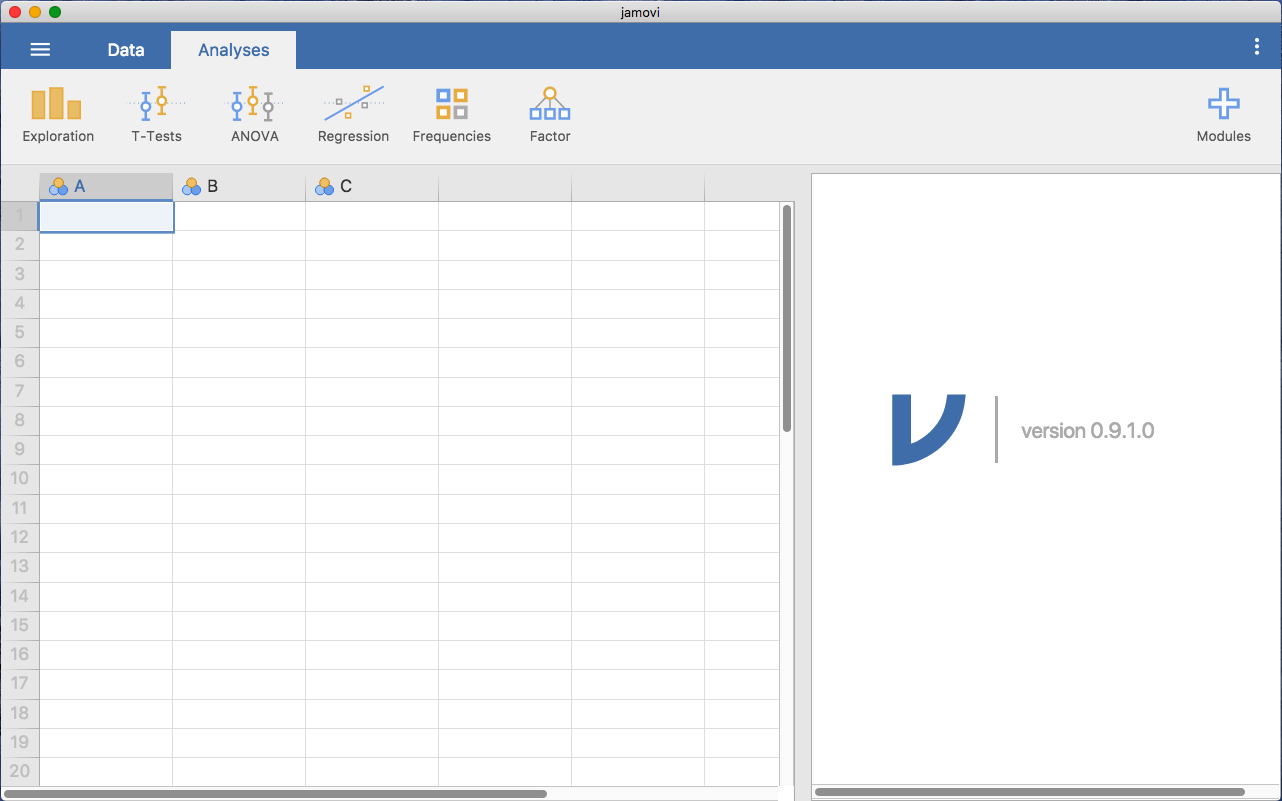
\epsfig{file=../img/introj/startingjamovi.png,clip=true,width=14cm}
\caption{jamovi looks like this when you start it.}
%\HR
\label{fig:startingjamovi}
\end{center}
\end{figure}

To the left is the spreadsheet view, and to the right is where the results of statistical tests appear. Down the middle is a bar separating these two regions, and this can be dragged to the left or the right to change their sizes. 

It is possible to simply begin typing values into the jamovi spreadsheet as you would any other spreadsheet software. Alternatively, existing data sets in the CSV (.csv) file format can be opened in jamovi. Additionally, you can easily import SPSS, SAS, Stata and JASP files directly into jamovi. To open a file, select the File tab (three horizontal lines signify this tab) at the top left hand corner, select ‘Open’ and then choose from the examples listed on 'Browse' depending on whether you want to open an example, or a file stored on your computer.


\section{Analyses\label{sec:analyses}}

Analyses can be selected from the analyses ribbon or menu along the top. Selecting an analysis will present an ‘options panel’ for that particular analysis, allowing you to assign different variables to different parts of the analysis, and select different options. At the same time, the results for the analysis will appear in the right ‘Results panel’, and will update as you make changes to the options.

When you have the analysis set up correctly, you can dismiss the analysis options by clicking the arrow to the top right of the optional panel. If you wish to return to these options, you can click on the results that were produced. In this way, you can return to any analysis that you (or say, a colleague) created earlier.

If you decide you no longer need a particular analysis, you can remove it with the results context menu. Right-clicking on the analysis results will bring up a menu, and by selecting ‘Analysis’, and then ‘Remove’, the analysis can be removed. But more on this later. First, let's take a more detailed look at the spreadsheet view.


\section{The spreadsheet\label{sec:spreadsheet}}

In jamovi, data is represented in a spreadsheet, with each column representing a ‘variable’.

\SUBSECTION{Data variables}

The most commonly used variables in jamovi are ‘Data Variables’, these variables simply contain data either loaded from a data file, or ‘typed in’ by the user. Data variables can be one of three measurement levels:

\begin{figure}[ht]
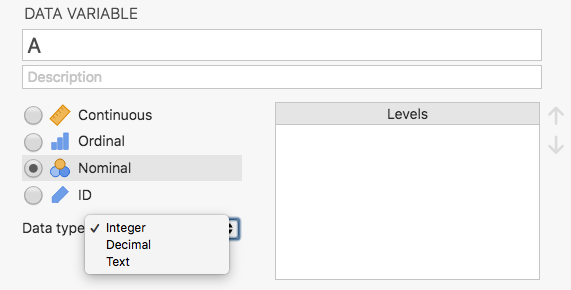
\epsfig{file=../img/introj/measurementlevels.png}
\end{figure}

These levels are designated by the symbol in the header of the variable’s column.

{\it Nominal} variables are for categorical variables which are text labels, for example a column called Gender with the values Male and Female would be nominal. So would a person’s name. Nominal variable values can also have a numeric value. These variables are used most often when importing data which codes values with numbers rather than text. For example, a column in a dataset may contain the values 1 for males, and 2 for females. It is possible to add nice ‘human-readable’ labels to these values with the variable editor (more on this later).

{\it Ordinal} variables are like Nominal variables, except the values have a specific order. An example might be a Likert scale, with 3 being ‘strongly agree’, and -3 being ‘strongly disagree’.

{\it Continuous} variables are variables which exist on a continuous scale. Examples might be height or weight. This is also referred to as ‘Interval’ or ‘Ratio scale’.

In addition, you can also specify different data types: variables have a data type of either ‘Text’, ‘Integer’ or ‘Decimal’. 

When starting with a blank spreadsheet and typing values in, the variable type will change automatically depending on the data you enter. This is a good way to get a feel for which variable types go with which sorts of data. Similarly, when opening a data file, jamovi will infer the variable type from the data in each column. In both cases, this automatic approach may not be correct, and it may be necessary to manually specify the variable type with the variable editor.

The variable editor can be invoked by selecting ‘Setup’ from the data tab or by double-clicking on the column header. The variable editor allows you to change the name of the variable, and (for data variables) the variable type, the order of the levels, and the label displayed for each level. Changes can be applied by clicking the ‘tick’ to the top right. The variable editor can be dismissed by clicking the `Hide' arrow.

New variables can be inserted or appended to the data set using the ‘add’ button from the data ribbon. The ‘add’ button also allows the addition of computed variables.


\SUBSECTION{Computed variables}

Computed Variables are those which take their value by performing a computation on other Variables. Computed Variables can be used for a range of purposes, including log transforms, z-scores, sum-scores, negative scoring and means.

Computed variables can be added to the data set, with the ‘add’ button available on the data tab. This will produce a formula box where you can specify the formula. The usual arithmetic operators are available. Some examples of formulas are:

A + B

LOG10(len)

MEAN(A, B)

(dose - VMEAN(dose)) / VSTDEV(dose)

In order, these are the sum of A and B, a log (base 10) transform of len, the mean of A and B, and the z-score of the variable dose. Figure \ref{fig:computedvariable} below shows the jamovi screen for the new variable computed as the z-score of dose (from the `Tooth Growth' example data set).

\vspace*{1cm}
\begin{figure}[ht]
\begin{center}
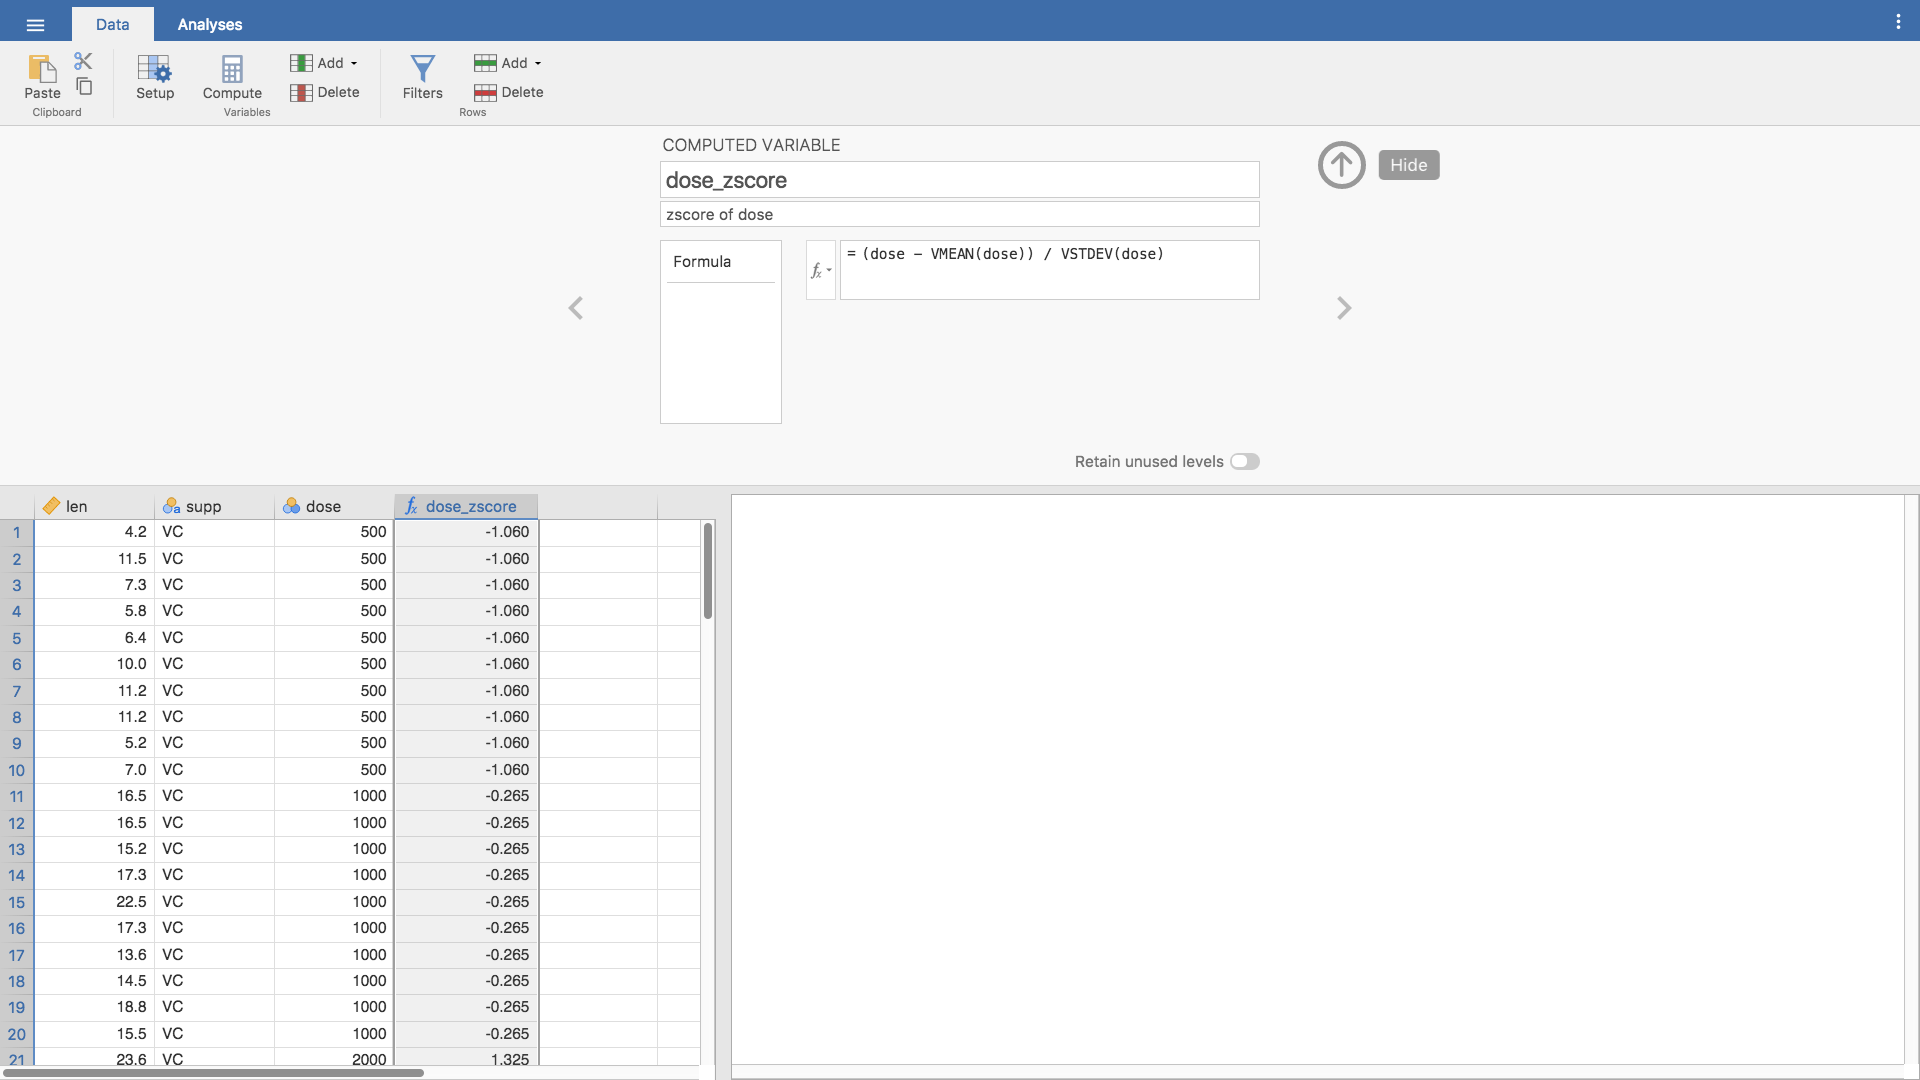
\epsfig{file=../img/introj/computedvariable.png,clip=true,width=14cm}
\caption{A newly computed variable, the z-score of `dose'.}
%\HR
\label{fig:computedvariable}
\end{center}
\end{figure}


{\it V-functions}

Many functions are already available in jamovi, available from the drop down box labelled {\it f\textsubscript{x}} . A number of functions appear in pairs, one prefixed with a V and the other not. V functions perform their calculation on a variable as a whole, where as non-V functions perform their calculation row by row. For example, MEAN(A, B) will produce the mean of A and B for each row. Where as VMEAN(A) gives the mean of all the values in A.

\SUBSECTION{Copy and Paste\label{sec:copypaste}}

jamovi produces nice APA formatted tables, and attractive plots. It is often useful to be able to copy and paste these, perhaps into a Word document, or into an email to a colleague. To copy results, right click on the object of interest, and from the menu select exactly what you want to copy. The menu allows you to choose to copy, say only the image, or the entire analysis. Selecting copy, copies the content to the clipboard, and can be pasted into the other program in the usual way. You can practice this later on when we do some analyses.

\SUBSECTION{Syntax mode\label{sec:syntaxmode}}

jamovi also provides an “\R\ Syntax Mode”, in this mode, jamovi produces equivalent \R\ code for each analysis. To change to syntax mode, select the Application menu to the top right of jamovi (a button with three vertical dots), and check the “Syntax mode” checkbox there. It is possible to leave syntax mode by clicking this a second time.

In syntax mode, analyses continue to operate as before, but now they produce \R\ syntax, and ‘ascii output’ like an \R\ session. Like all results objects in jamovi, you can right click on these items (including the \R\ syntax) and copy and paste them, for example, into an \R\ session. At present, the provided \R\ syntax does not include the data import step, and this must be performed manually. There are many resources explaining how to import data into \R\, and we recommend you take a look at these (Most analyses in jamovi require data as a data frame).

\section{Quitting jamovi \label{sec:quittingjamovi}}


There's one last thing I should cover in this chapter: how to quit jamovi. It's not hard, just close the program the same way you would any other program. However, what you might want to do before you quit is save your work! There are two parts to this: saving any changes to the data set, and saving the analyses that you ran.

It is good practice to save any changes to the data set as a new data set. That way you can always go back to the original data. To save any changes in jamovi, select `Export'...`Data' from the main jamovi menu (button with three horizontal bars in the top left and create a new file name for the changed data set.

Alternatively, you can save {\it both} the changed data and any analyses you have undertaken by saving as a jamovi file. To do this, from the main jamovi menu select `Save as' and type in a file name for this `jamovi file (.omv)'. Remember to save the file in a location where you can find it again later. I usually create a new folder for specific data sets and analyses.  


\section{Summary}

Every book that tries to a new statistical software program to novices has to cover roughly the same topics, and in roughly the same order. Mine is no exception, and so in the grand tradition of doing it just the same way everyone else did it, this chapter covered the following topics:

\begin{itemize}
\item {\it Getting started}. We downloaded and installed jamovi, and started it up (Section~\ref{sec:gettingjamovi}).
\item {\it Analyses}. We very briefly oriented to the part of jamovi where analyses are done and results appear, but then deferred this until later in the book (Section~\ref{sec:analyses}).
\item {\it The spreadsheet}. We spent more time looking at the spreadsheet part of jamovi, and considered different variable types, and how to compute new variables (Section~\ref{sec:analyses}).
\item {\it Quitting}. Finally, we looked at good practice in terms of saving your data set and analyses when you have finished and about to quit jamovi (Section~\ref{sec:quittingjamovi}).

\end{itemize}

\noindent
We still haven't arrived at anything that resembles data analysis. Maybe the next Chapter will get us a bit closer\ldots



